%%%%%%%%%%%%%%%%%%%%%%%%%%%%%%%%%%%%%%%%%%%%%%%%%%%%%%%%%%%%%%%%%%%%%%%%%%%%
% AGUJournalTemplate.tex: this template file is for articles formatted with LaTeX
%
% This file includes commands and instructions
% given in the order necessary to produce a final output that will
% satisfy AGU requirements, including customized APA reference formatting.
%
% You may copy this file and give it your
% article name, and enter your text.
%
%
% Step 1: Set the \documentclass
%
%

%% To submit your paper:
\documentclass[draft]{agujournal2019}
\usepackage{url} %this package should fix any errors with URLs in refs.
\usepackage{lineno}
\usepackage[inline]{trackchanges} %for better track changes. finalnew option will compile document with changes incorporated.
\usepackage{soul}
\linenumbers
%%%%%%%
% As of 2018 we recommend use of the TrackChanges package to mark revisions.
% The trackchanges package adds five new LaTeX commands:
%
%  \note[editor]{The note}
%  \annote[editor]{Text to annotate}{The note}
%  \add[editor]{Text to add}
%  \remove[editor]{Text to remove}
%  \change[editor]{Text to remove}{Text to add}
%
% complete documentation is here: http://trackchanges.sourceforge.net/
%%%%%%%

\draftfalse

%% Enter journal name below.
%% Choose from this list of Journals:
%
% JGR: Atmospheres
% JGR: Biogeosciences
% JGR: Earth Surface
% JGR: Oceans
% JGR: Planets
% JGR: Solid Earth
% JGR: Space Physics
% Global Biogeochemical Cycles
% Geophysical Research Letters
% Paleoceanography and Paleoclimatology
% Radio Science
% Reviews of Geophysics
% Tectonics
% Space Weather
% Water Resources Research
% Geochemistry, Geophysics, Geosystems
% Journal of Advances in Modeling Earth Systems (JAMES)
% Earth's Future
% Earth and Space Science
% Geohealth
%
% ie, \journalname{Water Resources Research}

\journalname{Water Resources Research}


\begin{document}
%TC:ignore
%% ------------------------------------------------------------------------ %%
%  Title
%
% (A title should be specific, informative, and brief. Use
% abbreviations only if they are defined in the abstract. Titles that
% start with general keywords then specific terms are optimized in
% searches)
%
%% ------------------------------------------------------------------------ %%

% Example: \title{This is a test title}

\title{Geometric models overestimate lake depth due to imperfect slope
measurement}

%% ------------------------------------------------------------------------ %%
%
%  AUTHORS AND AFFILIATIONS
%
%% ------------------------------------------------------------------------ %%

% Authors are individuals who have significantly contributed to the
% research and preparation of the article. Group authors are allowed, if
% each author in the group is separately identified in an appendix.)

% List authors by first name or initial followed by last name and
% separated by commas. Use \affil{} to number affiliations, and
% \thanks{} for author notes.
% Additional author notes should be indicated with \thanks{} (for
% example, for current addresses).

% Example: \authors{A. B. Author\affil{1}\thanks{Current address, Antartica}, B. C. Author\affil{2,3}, and D. E.
% Author\affil{3,4}\thanks{Also funded by Monsanto.}}

\authors{J. Stachelek\affil{1}, P. J. Hanly\affil{1}, and P. A. Soranno\affil{1}}

\affiliation{1}{Department of Fisheries and Wildlife, Michigan State University, 480
Wilson Rd., East Lansing, MI 48824, USA}
% \affiliation{2}{Second Affiliation}
% \affiliation{3}{Third Affiliation}
% \affiliation{4}{Fourth Affiliation}

% \affiliation{=number=}{=Affiliation Address=}
%(repeat as many times as is necessary)

%% Corresponding Author:
% Corresponding author mailing address and e-mail address:

% (include name and email addresses of the corresponding author.  More
% than one corresponding author is allowed in this LaTeX file and for
% publication; but only one corresponding author is allowed in our
% editorial system.)

% Example: \correspondingauthor{First and Last Name}{email@address.edu}

\correspondingauthor{J. Stachelek}{stachel2@msu.edu}

%% Keypoints, final entry on title page.

%  List up to three key points (at least one is required)
%  Key Points summarize the main points and conclusions of the article
%  Each must be 140 characters or fewer with no special characters or punctuation and must be complete sentences

% Example:
% \begin{keypoints}
% \item	List up to three key points (at least one is required)
% \item	Key Points summarize the main points and conclusions of the article
% \item	Each must be 140 characters or fewer with no special characters or punctuation and must be complete sentences
% \end{keypoints}

\begin{keypoints}
\item Geometric models to predict lake depth, which require in-lake slope, assume that nearshore land slope is a good proxy for in-lake slope.
\item Using data from thousands of lakes, we show that nearshore land slope is a poor proxy for in-lake slope and increases prediction error.
\item Prediction errors were systematic such that depth was overpredicted in concave and reservoir lakes.
\end{keypoints}

%% ------------------------------------------------------------------------ %%
%
%  ABSTRACT and PLAIN LANGUAGE SUMMARY
%
% A good Abstract will begin with a short description of the problem
% being addressed, briefly describe the new data or analyses, then
% briefly states the main conclusion(s) and how they are supported and
% uncertainties.

% The Plain Language Summary should be written for a broad audience,
% including journalists and the science-interested public, that will not have
% a background in your field.
%
% A Plain Language Summary is required in GRL, JGR: Planets, JGR: Biogeosciences,
% JGR: Oceans, G-Cubed, Reviews of Geophysics, and JAMES.
% see http://sharingscience.agu.org/creating-plain-language-summary/)
%
%% ------------------------------------------------------------------------ %%
%TC:endignore
%% \begin{abstract} starts the second page
\begin{abstract}
Lake depth is a critical characteristic that influences many important ecological processes in lakes. Unfortunately, lake depth measurements are labor-intensive to gather and are only available for a small fraction of lakes globally. Therefore, scientists have tried to predict lake depth from characteristics that are easily obtained for all lakes such as lake surface area or the slope of the land surrounding a lake. One approach for predicting lake depth simulates lake basins using a geometric model where nearshore land slope is assumed to be a representative proxy for in-lake slope and the distance to the center of the lake is assumed to be a representative proxy for the distance to the deepest point of the lake. However, these assumptions have rarely been tested in a broad range of lakes. We used bathymetry data from approximately 5,000 lakes and reservoirs to test these assumptions and to examine whether differences in lake type or shape influences depth prediction error. We found that nearshore land slope was not representative of in-lake slope and using it for prediction increases error substantially relative to models using true in-lake slope. We also found that models using nearshore land slope as a proxy systematically overpredict lake depth in concave lakes (i.e. bowl-shaped; up to 18\% of lakes in the study population) and reservoir lakes (up to 30\% of lakes in the study population), suggesting caution in using geometric models for depth prediction in unsampled lakes.
\end{abstract}

%% ------------------------------------------------------------------------ %%
%
%  TEXT
%
%% ------------------------------------------------------------------------ %%

%%% Suggested section heads:
% \section{Introduction}
%
% The main text should start with an introduction. Except for short
% manuscripts (such as comments and replies), the text should be divided
% into sections, each with its own heading.

% Headings should be sentence fragments and do not begin with a
% lowercase letter or number. Examples of good headings are:

% \section{Materials and Methods}
% Here is text on Materials and Methods.
%
% \subsection{A descriptive heading about methods}
% More about Methods.
%
% \section{Data} (Or section title might be a descriptive heading about data)
%
% \section{Results} (Or section title might be a descriptive heading about the
% results)
%
% \section{Conclusions}


\section{Introduction}
\noindent
\noindent
Lake depth is an important factor controlling lake physics, chemistry, and biota. Deeper lakes generally have higher water clarity and less complete mixing compared to shallow lakes \cite{feeEffectsLakeSize1996, readSimulating2368Temperate2014}. These differences are reflected in variation among lakes in terms of biological productivity \cite{qinWaterDepthUnderpins2020} and rates of greenhouse gas production \cite{liSignificantContributionLake2020}. However, because measured depth data is only available for a small fraction ($\sim$25\%) of all lakes, our ability to understand and predict depth-dependent processes is limited. The importance of lake depth, coupled with its limited availability, has led to numerous attempts to predict depth using measures available for all lakes such as lake surface area or the nearshore slope of the land surrounding a lake \cite{heathcotePredictingBathymetricFeatures2015, oliver2016prediction, sobekPredictingDepthVolume2011}. Given the limited prediction accuracy of prior depth prediction efforts ($\pm$ 6-7 m), a major focus has been on  improving prediction accuracy using strategies such as employing more diverse covariates \cite{oliver2016prediction}, varying lake buffer sizes \cite{heathcotePredictingBathymetricFeatures2015}, or estimating hidden groupings (e.g. fitting different models for distinct size classes) among lakes \cite{sobekPredictingDepthVolume2011}.

One approach for predicting lake depth involves using a geometric model that assumes lake basins correspond to an idealized shape such as a cone, bowl, or an elliptic sinusoid \cite{hollisterPredictingMaximumLake2011, neumannMaximumDepthAverage1959, yigzawNewGlobalStorage2018}. All such geometric models for lake depth prediction involve implicit assumptions about the terms of geometric formulae. In the simplest case, where lakes basins are treated as cones (Equation \ref{eq1}, Figure \ref{fig1}), two assumptions are required to make depth predictions for all lakes: 1) that nearshore land slope is a representative proxy for in-lake slope and 2) that the distance to the center of the lake is a representative proxy for the distance to the deepest point of the lake (Figure \ref{fig1}). This cone model imposes the following fixed (i.e. geometric) relationship between slope and horizontal distance:

\begin{linenomath*}
\begin{equation}
      depth_{geometric} = tan(slope) * distance \label{eq1}
\end{equation}
\end{linenomath*}

\noindent
where the product of slope and horizontal distance yields an exact geometric depth estimate ($depth_{geometric}$).

\begin{figure}
\noindent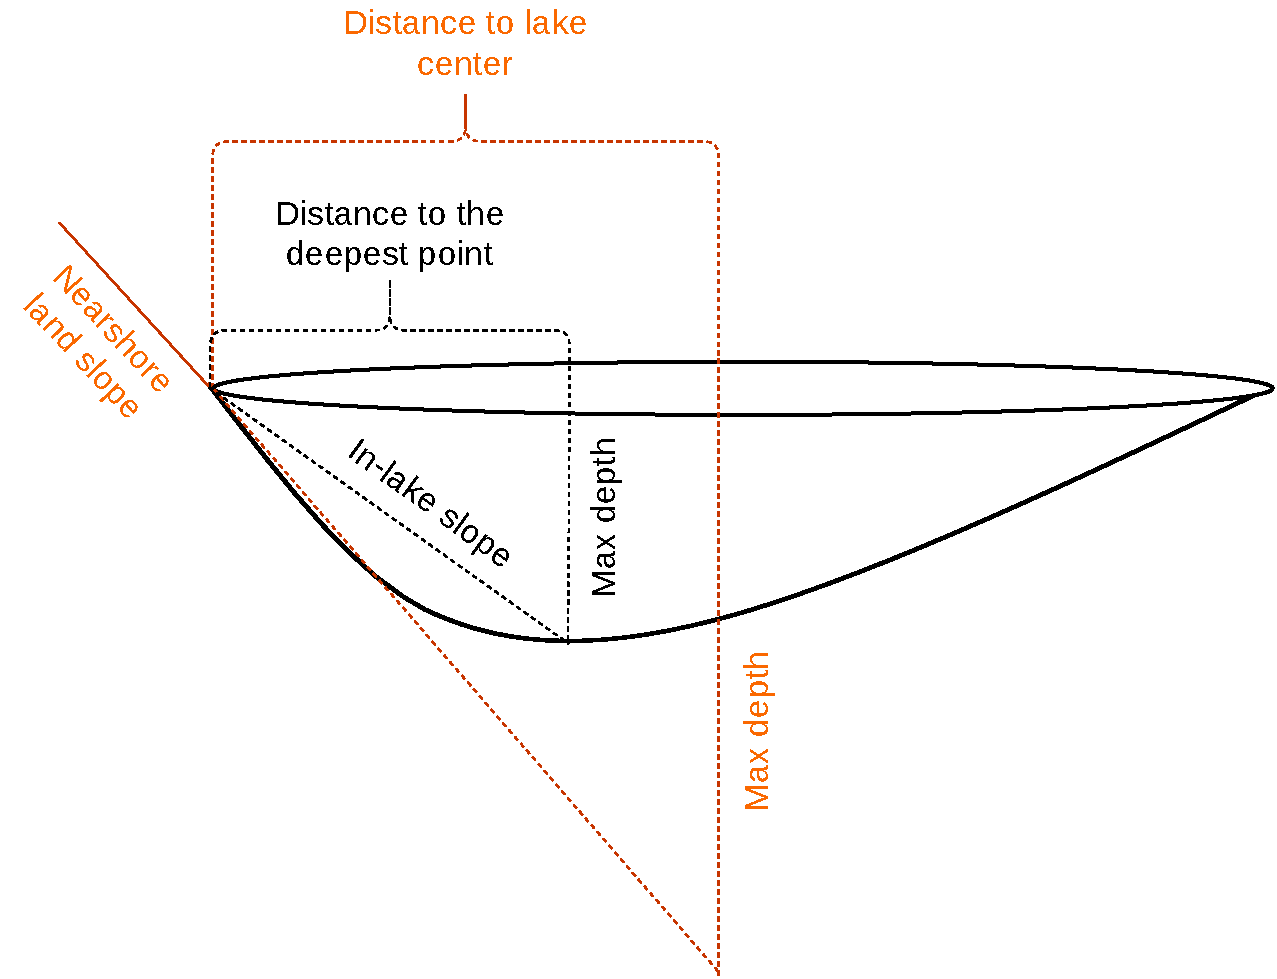
\includegraphics[width=0.85\textwidth]{../figures/slope_diagram_new}
\caption{Diagram showing the relations between true (black) and proxy (orange) metrics of lake geometry. Geometric depth calculated via Equation \ref{eq1} requires a single distance and slope metric.}\label{fig1}
\end{figure}

The assumptions of the cone model (as well as other geometric models) can be tested by comparing proxy measures of lake geometry against corresponding “true” (i.e. in-lake) values derived from bathymetric maps and by evaluating how lake cross-section shapes differ from that of an idealized cone \cite{johanssonNewApproachesModelling2007}. For instance, lake cross-section shapes have been shown to vary from narrow "convex" forms to outstretched "concave" forms \cite{hakansonLakeFormLake1977}. Because tests of geometric model assumptions require bathymetric map data, which is only available for about 15\% of all lakes, existing evidence may not be applicable to all lakes. The few studies that have tested these assumptions have been limited to individual studies of very large ($>$ 500 ha) lakes or studies on small numbers ($<$ 100) of lakes \cite{johanssonNewApproachesModelling2007}. Studies focused specifically on reservoirs (as opposed to the more typical case where reservoirs and natural lakes are combined), have been even more restricted to that of extremely large lakes $>$ 1000 ha \cite{lehnerHighresolutionMappingWorld2011, messagerEstimatingVolumeAge2016}.

As a result of this limited testing, we lack knowledge on both the predictive performance of geometric models, the effect of proxies on depth prediction, and whether depth predictions are more sensitive to measurement errors in the horizontal dimension (i.e. distance to the deepest point of the lake) or measurement errors in the vertical dimension (i.e. in-lake slope). Additionally it is unclear whether model prediction error is related to differences in lake type such those with different cross-section shapes or those classified as reservoirs versus natural lakes. Given these knowledge gaps, we asked three research questions: 1) How representative is nearshore land slope of in-lake slope; and how representative is the distance to the center of a lake compared to the distance to the deepest point of a lake? 2) How does the use of proxies for lake geometry affect lake depth prediction error? 3) How does lake cross-section shape (i.e. concave versus convex) and lake type (i.e. natural lake vs reservoir) affect depth prediction error? To answer these questions, we extracted maximum depth (hereafter referred to as “observed maximum depth”), in-lake slope, cross-section shape (i.e., concave versus convex), and distance to the deepest point, of approximately 5,000 lakes from bathymetric map data and supplemented this data with classification estimates of whether lakes are reservoirs or natural lakes. We used this data to compute geometric depth estimates (Equation \ref{eq1}) and prediction "offsets" to these estimates using the random forest algorithm (Equation \ref{eq3}). Covariates used in offset modeling included a variety of lake, watershed, and hydrologic subbasin measures that are available for all lakes (Table S1).

By definition, the distance proxy (distance to the center of the lake) must always be greater or equal to the true distance value (distance to the deepest point of the lake). Therefore, we expect that the use of this proxy will lead to overestimation of lake depth (Figure \ref{fig1}). Furthermore we expect to see greater overestimation error in reservoirs as compared to natural lakes because many reservoirs are known to be drowned river valleys where the deepest point is close to the edge at the end of the reservoir (i.e. next to the dam) rather than in the center of the reservoir \cite{lanza1985interactions}. In a similar fashion, we expect to see overestimation error associated with using a nearshore land slope proxy in lakes with differing cross-section shape such that the depth of U-shaped (i.e. concave) lakes will be overpredicted whereas the depth of V-shaped (i.e. convex) lakes will be underpredicted (Figure S1). Finally, we expect that depth predictions themselves will be strongly related to lake area and hydrologic subbasin variables as these measures have been influential in prior studies \cite{oliver2016prediction}.

By testing these expectations, we can establish whether barriers to increased depth prediction accuracy lie in lack of correspondence between true and proxy measures of lake geometry or in hidden groupings among lakes (such as lake cross-section shape or reservoir status). This information could help direct future research efforts to focus on particular dimensions of lake geometry (i.e. horizontal versus vertical) or to stratify model predictions based on specific lake types and cross-section shapes. Ultimately, achieving increased depth prediction accuracy would allow for more precise estimates of depth-dependent biotic and chemical processes across broad spatial extents.

\section{Methods}
\subsection{Data description}
\noindent
We compiled bathymetry data on approximately 5,000 lakes in the Northeastern and Midwestern US from nine official state databases (Figure S2). The original data came in a variety of formats including pre-interpolated rasters (Minnesota), contour lines (Nebraska, Michigan, Massachusetts, Kansas, Iowa), contour polygons (New Hampshire, Connecticut), or point depth soundings (Maine). For the Minnesota data, we simply clipped the raster for each lake to its outline. For data from the remaining states, we processed each lake by converting its original representation to a point layer (if necessary), rasterizing these points, and creating an interpolated bathymetry “surface” using a simple moving window average in the \texttt{raster} R package \cite{hijmansRasterGeographicData2019}. The size of the moving window was adjusted iteratively to ensure that each bathymetry raster contained no missing data.

All lake bathymetry was specifically calculated relative to high-resolution (1:24,000 scale) NHD \cite{usgsNationalHydrographyDataset2019} waterbodies such that source data and bathymetry surface outputs were clipped to the area of each lake polygon. We restricted the lakes in our study to those with an area of at least 4 ha and a maximum depth of at least 0.3 m (1 ft). The purpose of these restrictions was to ensure that lakes had enough contours (or points, or polygons) to generate adequately smooth interpolations with which to calculate in-lake geometry metrics.

We used our generated bathymetry surfaces to find the location of the deepest point in the lake and we resolved ties by choosing the deepest point that was closest to the center of the lake. We calculated the center of the lake not as its centroid but rather by finding the point farthest from the lake shoreline (i.e. its “visual distance to lake center”). For these calculations, we used the \texttt{polylabelr} R package \cite{larssonPolylabelrFindPole2019}, which interfaces with the Mapbox pole of inaccessibility algorithm \cite{agafonkinJSLibraryFinding2019}. We calculated in-lake slope as maximum lake depth divided by the distance to the deepest point and we calculated nearshore land slope for each lake by computing the slope within a 100-m buffer using data from a high resolution digital elevation model ($\sim$15x15m grain) accessed using the \texttt{elevatr} R package \cite{hollisterElevatrAccessElevation2017} and computed using the terrain function in the \texttt{raster} R package \cite{hijmansRasterGeographicData2019}.

We categorized lakes based on their cross-section shape and reservoir class. For cross-section shape, we categorized lakes as either convex or concave following the method of \citeA{hakansonLakeFormLake1977} by computing normalized lake depth-area relationships (i.e. hypsographic curves) and assigning class membership based on whether a lake’s curve falls above or below that of a simple straight-sided cone (Figure S3). We further classified lakes using the output of a machine learning algorithm to assign a probability to each lake as to whether it is a reservoir or a natural lake. For our purposes, we determined a lake to be a reservoir if the classification probability was 0.75 or greater. Our reservoir classification data defines reservoirs as any permanent waterbody that has a water control structure likely to significantly impact flow or pool water, beyond simply controlling water level. It makes no distinction between different dam types or dam heights.

Covariates used in random forest modeling (Table S1, Equation \ref{eq3}) for lake elevation, area, island area, perimeter, shoreline development, watershed to lake area ratio, and hydrologic subbasin (i.e. HUC4s), were obtained from the LAGOS-US LOCUS database. One such measure, that of shoreline development, is a measure of lake perimeter shape defined as:

\begin{linenomath*}
      \begin{equation}
            shoreline_{devel} = perimeter / (2 * \sqrt{(\pi * waterarea * 10000)}) \label{eq2}
      \end{equation}
      \end{linenomath*}

\noindent
where sinuous lakes have larger values of shoreline development and circular lakes have smaller values of shoreline development. Watershed to lake area ratio is an approximation of water residence time and is defined as watershed area divided by lake area.

\subsubsection{Proxy evaluation}
\noindent
We conducted a qualitative assessment of whether or not proxy measures of lake geometry are representative of their true values by visual inspection (i.e. plotting each proxy measure against its corresponding true value) and by computing coefficients of determination ($R^2$). We further tested proxy measures by examining their effect on lake depth prediction error. Our approach involved several steps. In the first step, we computed a geometric estimate of lake depth using only geometry information ($depth_{geometric}$, Equation \ref{eq1}). In the second step, we fit a random forest model to predict observed (i.e. true) depth as a function of geometric depth along with several covariates available for all lakes (Table S1). The purpose of this random forest “offset” modeling was to more rigorously test our expectations regarding prediction error among different formulations of $depth_{geometric}$ and among different lake types. Each of these steps were executed iteratively for each combination of true and proxy values of slope and distance (Table \ref{table2}).

\subsection{Model description}
\subsubsection{Geometric model}
\noindent
We used a geometric model of lakes where basins are treated as cones with a fixed relationship between slope and distance (Equation \ref{eq1}). Note that Equation \ref{eq1} is a geometric formula and has no intercept or “coefficients” and it produces a perfect depth estimate given true values of slope and distance. To use this model to predict the depth of all lakes, there is a necessary assumption that proxy slope and distance measures, which are available for all lakes, are representative of true slope and distance (Figure \ref{fig1}).

\subsubsection{Random forest models}
\noindent
Prior studies using geometric models to predict lake depth include a statistical or machine learning model “layer” or “offset” to boost predictive accuracy. For our purposes, this offset modeling enabled us to test our expectations that prediction error would be different among different formulations of $depth_{geometric}$ and among different lake types. It also facilitated direct comparison against prior models of lake depth including those that are non-geometric. We generated an “offset” to geometric depth \cite<sensu>{hollisterPredictingMaximumLake2011} using the random forest algorithm and the \texttt{ranger} R package \cite{wrightRangerFastImplementation2017} to predict observed maximum depth as a function of covariates including geometric maximum depth (from Equation \ref{eq1}) along with the lake elevation, area, perimeter, and ratio/index measures listed in Table 1:

\begin{linenomath*}
      \begin{equation}
            depth_{observed} \sim depth_{geometric} + covariates \label{eq3}
      \end{equation}
      \end{linenomath*}

\noindent
Neither cross-section shape nor reservoir class was used as a covariate in any random forest models. We used the random forest algorithm because it makes no assumptions about the distribution of model residuals, allows for non-linearity, and is insensitive to interactions (i.e. multicollinearity) among covariates \cite{prasadNewerClassificationRegression2006}.

\subsubsection{Model comparisons}
\noindent
We tested model sensitivity to slope and distance proxies by generating multiple “geometric maximum depth” estimates from 3 different model runs using each of the possible metric combinations for Equation \ref{eq1} (true slope - proxy distance, proxy slope - true distance, proxy slope - proxy distance). Prior to entry into Equation \ref{eq1}, we standardized proxy distances to have the same numeric range as their true counterpart. The purpose of this standardization was to prevent lakes with extremely long proxy distances from having an outsized impact on model evaluation metrics.

\subsubsection{Model evaluations}
\noindent
We evaluated model fit and prediction error using root-mean-square error (RMSE) and coefficient of determination ($R^2$) metrics on a holdout set containing 25\% of all lakes. We evaluated the residuals of each model relative to lake cross-section shape and reservoir classes to determine whether depth is consistently over or under predicted for some lake types relative to others.

\section{Results}
\noindent
Lakes belonging to each cross-section shape and reservoir class were not evenly distributed across our study area (Figure S2, S3). For example, concave lakes were nearly absent from Michigan whereas Maine lakes had an overabundance of lakes categorized as neither concave nor convex. Lakes in the southern portions of our study area tended to be classified as reservoirs whereas lakes in the northern portions of our study area were a more even mix between reservoirs and natural lakes (Figure S2). Approximately 18\%, 80\%, and 2\% of lakes were classified as having a concave, convex, or neither shape respectively whereas approximately 30\% and 70\% of lakes were classified as being a reservoir or a natural lake.

Although proxy distance to lake center was often much larger in magnitude compared to the true distance to the deepest point of lakes’, they were strongly related ($R^2$ = 0.8). In contrast, proxy nearshore land slope and true in-lake slope were more weakly related ($R^2$ = 0.17). For slope measures, most lakes had lower magnitude (i.e. shallower) nearshore land slope compared to true in-lake slope (Figure \ref{fig3}). Taken together, these results suggest that proxy distance to the center of lakes is representative of true distance to the deepest point of lakes whereas proxy nearshore land slope is not representative of true in-lake slope. In addition to overall differences between slope and distance measures, we found differences in these relationships among lake shape classes. For example, in-lake slope and distance to the deepest point of the lake metrics were consistently larger in magnitude for convex lakes as compared to concave lakes (Figure S4). However,  there were not similar differences among slope and distance metrics for natural lakes versus reservoirs (Figure S4).

\begin{figure}
  \begin{center}
    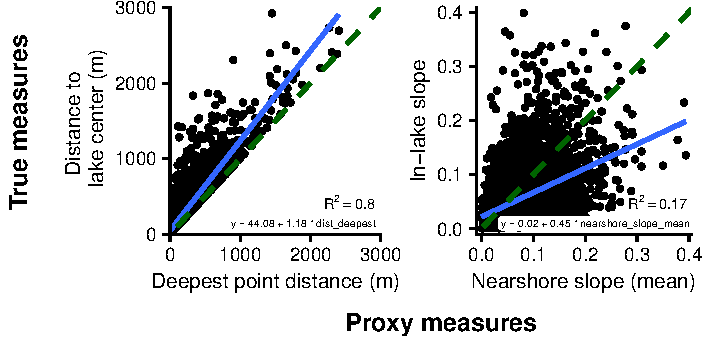
\includegraphics[width=0.75\textwidth,keepaspectratio]{../figures/01_geometry_base-1}
  \end{center}
  \caption{Comparison among proxy and true values of lake geometry for A) distance to deepest point versus distance distance to lake center and B) nearshore land slope versus in-lake slope. A best-fit line and coefficient of determination is shown to illustrate representativeness.}\label{fig3}
\end{figure}

The use of proxy nearshore land slope had a larger effect on model fit and prediction error than the use of proxy distance to lake center (Table \ref{table2}). More specifically, the true slope - proxy distance model had a better fit ($R^2$ = 0.73) and lower prediction error (RMSE = 4.23m) compared to the proxy slope - true distance model ($R^2$ = 0.26, RMSE = 6.87m). Furthermore, analysis of model residuals showed overestimation of lake depth for concave lakes when models included a proxy slope measure (Figure \ref{fig4}). We observed similar but smaller overestimation depending on if a lake was classified as a reservoir rather than a natural lake (Figure \ref{fig4}).

\begin{table}[h]
  \caption{Model fit and predictive accuracy metrics (RMSE = root mean square error, $R^2$ = coefficient of determination) for all combinations of true (in-lake slope, distance to the deepest point of the lake) and proxy (nearshore land slope, distance to lake center) metrics.} \label{table2}
  \centering
  % \setlength\tabcolsep{1.5pt} % default value: 6pt
\begin{tabular}{llll}
  \hline
  slope & distance & RMSE & $R^2$\\
  \hline
  true & true & - & -\\
  true & proxy & 4.2 m & 0.73\\
  proxy & true & 6.9 m & 0.26\\
  proxy & proxy & 6.6 m & 0.31\\
  \hline
\end{tabular}
\end{table}

\begin{figure}
  \begin{center}
    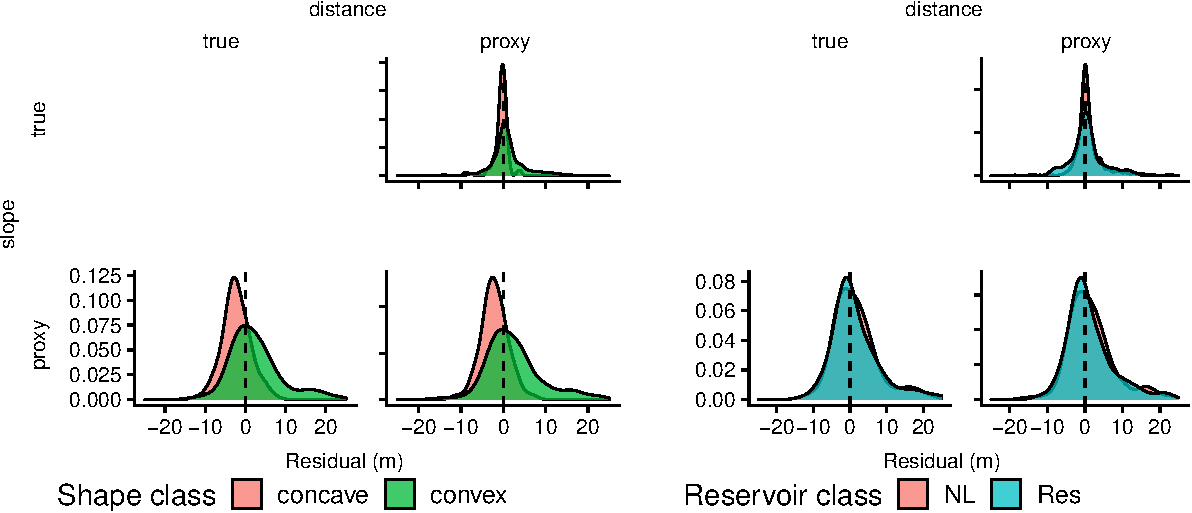
\includegraphics[width=\textwidth,keepaspectratio]{../figures/02_depth_model_grid_resid-1}
  \end{center}
  \caption{Depth model residuals (residual  = observed - predicted) in meters by cross-section shape and reservoir class indicating overprediction of concave and reservoir lakes.}\label{fig4}
\end{figure}

The most important covariates in offset models were those relating to spatial location, lake area, and perimeter (Figure S5). Conversely, watershed metrics and lake elevation had little contribution to random forest model fit (Figure S5). The spatial location (i.e. HUC4) covariate was notably less importance in the true slope model compared to the two proxy slope models. Model importance calculations indicated that omitting a geometric max depth measure results in a 130\%, 60\%, or 50\% increase in mean square error depending on the formulation of geometric max depth in Equation \ref{eq1} (Figure S5).

\section{Discussion}
\noindent
Our tests of geometric lake depth models show that specific proxy measures of lake geometry are not representative of true geometry measures across a broad array of lakes. Models using non-representative proxies showed increased error and systematic overestimation of depth in concave and reservoir lakes. Although our analysis was limited to lakes with available bathymetry data, these lakes did not have characteristics that differed from that of the overall lake population (Figure S6, S8). Although there is a possibility that there is some hidden bias not explored for in our analyses, this lack of difference suggests that our results are likely to be broadly applicable to all lakes.

\subsection{Representativeness of proxy measures of lake geometry}
\noindent
In comparing among lake geometry measures, our analysis suggests that proxy distance to lake center is representative of true distance to the deepest point of the lakes but that proxy nearshore land slope is not representative of true in-lake slope. A simple indication of this non representativeness is that proxy nearshore land slope was often (in $>$ 74\% of cases) steeper than true in-lake slope. This finding is consistent with \citeA{heathcotePredictingBathymetricFeatures2015} whos results suggest that in-lake slopes are shallower compared to the surrounding land. The shallow nature of in-lake slopes is likley a function of erosion and sediment transport processes \cite{hakansonLakeBottomDynamics1981, johanssonNewApproachesModelling2007}.

One surprising finding with respect to the relationship between true and proxy geometry measures when examined by lake class was the fact that there was no greater difference between proxy and true distances in reservoirs compared to natural lakes. This is contrary to the idea that most reservoirs are drowned river valleys where the deepest point is close to the edge at the end of the reservoir (i.e. next to the dam) rather than in the center of the reservoir \cite{lanza1985interactions}. One possible explanation is that our reservoir classification data uses a more general definition of a reservoir (i.e. any permanent waterbody that has a water control structure likely to significantly impact flow or pool water) compared to that of conventional classifications that are tied to specific dam types or dam heights. Another possible explanation is that conventional reservoir classifications are conceptually biased towards more southern areas with few natural lakes (Figure S2).

We found other differences among lake geometry measures according to lake cross-section shape. One finding was that convex lakes, when compared to concave lakes, had longer distances to lake centers relative to corresponding distances to the deepest point of lakes. In addition, convex lakes often had steeper in-lake slopes relative to nearshore land slopes as compared to concave lakes. Finally, it was notable that convex lakes were deeper than concave lakes despite having similar distributions of lake surface area (Figure S7). The underlying cause of these differences is unknown but one possibility is that geometry is tied to the circumstances of lake formation whereby the formation of concave lakes were a result of more intense glacial scouring compared to that of convex lakes \cite{gorhamPhysicalLimnologyNorthern1958}. While our findings provide some evidence in support of this idea, namely that there is a geographic hotspot of concave lakes associated with the glaciated “prairie pothole region” \cite<see>{hayashiSimpleEquationsRepresent2000}, the overall geographic distribution of lake cross-section shapes does not support this idea. Instead of a concentrated area of concave lakes in formerly glaciated regions, there appears to be a fairly even mix of concave and convex lakes distributed amongst the northern (i.e. glaciated) and southern (non-glaciated) portions of our study area (Figure S2).

\subsection{Effects of proxy measures of lake geometry depth prediction error}
\noindent
Models using only proxy variables had prediction error rates (RMSE = 6.6m) of a similar magnitude as that of prior studies (RMSE = 6 - 7.3m) predicting lake depth at broad geographic extents \cite{hollisterPredictingMaximumLake2011, oliver2016prediction, messagerEstimatingVolumeAge2016}. When only a single proxy measure was used, there was a difference in model sensitivity depending on if it was a horizontal distance measure or a vertical slope measure. In the case of a true slope and proxy distance combination, models were more accurate ($\pm$ 4.2m) than even the most accurate of prior studies \cite{hollisterPredictingMaximumLake2011, oliver2016prediction, messagerEstimatingVolumeAge2016}. Conversely, models using a proxy slope and true distance combination had prediction error rates ($\pm$ 6.9m) of a similar magnitude as that of the baseline proxy-proxy model ($\pm$ 6.6m). The greater sensitivity of depth predictions to proxy slope measures relative to proxy distance measures may be explained by the fact that proxy slope measures were a more imperfect representation of true in-lake slopes relative to proxy versus true distances. In addition, these results help explain the relatively poor predictive performance of prior non-geometric lake depth models given that they rely heavily on lake area as a predictor \cite{messagerEstimatingVolumeAge2016, oliver2016prediction, sobekPredictingDepthVolume2011} and both horizontal distance measures and vertical slope measures appear to be decoupled from lake area (Figure S7).

\subsection{Effects of lake shape and lake type on depth prediction error}
\noindent
As expected, we found that the maximum depth of concave lakes was systematically overpredicted by a simple geometric model using proxy nearshore land slope (Figure S1). However, contrary to our expectation, we did not observe underprediction of depth in convex lakes. The reason we did not observe underprediction of the depth of convex lakes is likely because geometric depth itself was always greater than observed maximum depth owing to the fact that proxy distance is constrained to be greater than true distance. This suggests that depth estimates in prior studies may be overestimated when they encompass large numbers of lakes with diverse cross-section shapes.

\subsection{Future research}
\noindent
One of our models (true slope, proxy distance) was more accurate than even the most accurate of prior studies. However, parameterization of this model requires data on bathymetry which is not available for all lakes. We propose that the error rate of this model ($\pm$ 4.2m) be used as an out-of-sample prediction benchmark for future studies such that they should attempt to match it but not expect to exceed it.

Because this most accurate model requires bathymetry data, this suggests that it may not be possible with current data and models to produce depth predictions for all lakes with error rates below 6m. To achieve high prediction accuracy using data available for all lakes, future studies could explore alternative modeling approaches such as ordinal modeling, which would capture whether or not a lake crosses some important depth threshold but would not seek to predict a specific depth value, or emerging data types such as “topobathymetric” products that integrate both topographic and bathymetric data in a seamless fashion rather than treating them as separate entities. Topobathymetry would allow for more robust tests of the representativeness of geometric model inputs. Unfortunately, topobathymetric products are rare, have mostly been limited nearshore marine environments, and as such are not yet widely available for inland waters \cite{danielsonTopobathymetricElevationModel2016}.

Finally, our findings indicate that geometry measures differ according to lake cross-section shape. This makes it an attractive target for inclusion in depth prediction models. Unfortunately, identifying a lake’s cross-section shape requires bathymetry data which is unavailable for most lakes. However, given the conceptual links between cross-section shape, glaciation, and sedimentation \cite{johanssonNewApproachesModelling2007} it may be advantageous for future studies to compile data on sedimentation to determine if this data can be used to predict cross-section shape and boost depth prediction accuracy.

\section{Conclusion}
\noindent
To our knowledge, the present study is the largest and most comprehensive test to date of geometric models of lake depth. Using bathymetry data on approximately 5,000 lakes, we show that proxy slope measures are not representative of true in-lake slope and this leads to inaccuracies in predicting the depth of concave and reservoir lakes. These innaccuracies suggest that caution is warranted in using geometric models for depth prediction in unsampled lakes. Despite these apparent biases, overall prediction accuracy was equivalent to that of prior depth prediction studies ($\pm$ 6-7m). Only our models using a true measure of in-lake slope, which is limited in availability to lakes with bathymetry data and where we already know lake depth, had greater accuracy than that of prior studies ($\pm$ 4.2m). Lack of improved prediction accuracy (short of including data that is unavailable for most lakes) suggests that improved prediction may require new types of data or novel analysis techniques.

%%

%% Enter Figures and Tables near as possible to where they are first mentioned:
%
% DO NOT USE \psfrag or \subfigure commands.
%
% Figure captions go below the figure.
% Table titles go above tables;  other caption information
%  should be placed in last line of the table, using
% \multicolumn2l{$^a$ This is a table note.}
%
%----------------
% EXAMPLE FIGURES
%
% \begin{figure}
% \includegraphics{example.png}
% \caption{caption}
% \end{figure}
%
% Giving latex a width will help it to scale the figure properly. A simple trick is to use \textwidth. Try this if large figures run off the side of the page.
% \begin{figure}
% \noindent\includegraphics[width=\textwidth]{anothersample.png}
%\caption{caption}
%\label{pngfiguresample}
%\end{figure}
%
%
% If you get an error about an unknown bounding box, try specifying the width and height of the figure with the natwidth and natheight options. This is common when trying to add a PDF figure without pdflatex.
% \begin{figure}
% \noindent\includegraphics[natwidth=800px,natheight=600px]{samplefigure.pdf}
%\caption{caption}
%\label{pdffiguresample}
%\end{figure}
%
%
% PDFLatex does not seem to be able to process EPS figures. You may want to try the epstopdf package.
%

%
% ---------------
% EXAMPLE TABLE
%
% \begin{table}
% \caption{Time of the Transition Between Phase 1 and Phase 2$^{a}$}
% \centering
% \begin{tabular}{l c}
% \hline
%  Run  & Time (min)  \\
% \hline
%   $l1$  & 260   \\
%   $l2$  & 300   \\
%   $l3$  & 340   \\
%   $h1$  & 270   \\
%   $h2$  & 250   \\
%   $h3$  & 380   \\
%   $r1$  & 370   \\
%   $r2$  & 390   \\
% \hline
% \multicolumn{2}{l}{$^{a}$Footnote text here.}
% \end{tabular}
% \end{table}

%% SIDEWAYS FIGURE and TABLE
% AGU prefers the use of {sidewaystable} over {landscapetable} as it causes fewer problems.
%
% \begin{sidewaysfigure}
% \includegraphics[width=20pc]{figsamp}
% \caption{caption here}
% \label{newfig}
% \end{sidewaysfigure}
%
%  \begin{sidewaystable}
%  \caption{Caption here}
% \label{tab:signif_gap_clos}
%  \begin{tabular}{ccc}
% one&two&three\\
% four&five&six
%  \end{tabular}
%  \end{sidewaystable}

%% If using numbered lines, please surround equations with \begin{linenomath*}...\end{linenomath*}
%\begin{linenomath*}
%\begin{equation}
%y|{f} \sim g(m, \sigma),
%\end{equation}
%\end{linenomath*}

%%% End of body of article

%%%%%%%%%%%%%%%%%%%%%%%%%%%%%%%%
%% Optional Appendix goes here
%
% The \appendix command resets counters and redefines section heads
%
% After typing \appendix
%
%\section{Here Is Appendix Title}
% will show
% A: Here Is Appendix Title
%
%\appendix
%\section{Here is a sample appendix}

%%%%%%%%%%%%%%%%%%%%%%%%%%%%%%%%%%%%%%%%%%%%%%%%%%%%%%%%%%%%%%%%
%
% Optional Glossary, Notation or Acronym section goes here:
%
%%%%%%%%%%%%%%
% Glossary is only allowed in Reviews of Geophysics
%  \begin{glossary}
%  \term{Term}
%   Term Definition here
%  \term{Term}
%   Term Definition here
%  \term{Term}
%   Term Definition here
%  \end{glossary}

%
%%%%%%%%%%%%%%
% Acronyms
%   \begin{acronyms}
%   \acro{Acronym}
%   Definition here
%   \acro{EMOS}
%   Ensemble model output statistics
%   \acro{ECMWF}
%   Centre for Medium-Range Weather Forecasts
%   \end{acronyms}

%
%%%%%%%%%%%%%%
% Notation
%   \begin{notation}
%   \notation{$a+b$} Notation Definition here
%   \notation{$e=mc^2$}
%   Equation in German-born physicist Albert Einstein's theory of special
%  relativity that showed that the increased relativistic mass ($m$) of a
%  body comes from the energy of motion of the body—that is, its kinetic
%  energy ($E$)—divided by the speed of light squared ($c^2$).
%   \end{notation}



%TC:ignore
%%%%%%%%%%%%%%%%%%%%%%%%%%%%%%%%%%%%%%%%%%%%%%%%%%%%%%%%%%%%%%%%
%
%  ACKNOWLEDGMENTS
%
% The acknowledgments must list:
%
% >>>>	A statement that indicates to the reader where the data
% 	supporting the conclusions can be obtained (for example, in the
% 	references, tables, supporting information, and other databases).
%
% 	All funding sources related to this work from all authors
%
% 	Any real or perceived financial conflicts of interests for any
%	author
%
% 	Other affiliations for any author that may be perceived as
% 	having a conflict of interest with respect to the results of this
% 	paper.
%
%
% It is also the appropriate place to thank colleagues and other contributors.
% AGU does not normally allow dedications.

\acknowledgments All data as well as code for data processing, model fitting, and model evaluation is available at [Zenodo DOI]. Funding was provided by the US NSF Macrosystems Biology Program grants, DEB-1638679; DEB-1638550, DEB-1638539, DEB-1638554. PAS was also supported by USDA National Institute of Food and Agriculture Hatch Project, Grant Number: 176820. Author contributions: JS conceived of the study, built models, analyzed data, and wrote the paper. PJH and PAS provided interpretation of results and edited the paper. This work benefited from participation in the Global Lake Ecological Observatory Network (GLEON). We thank K.S. Cheruvelil for a friendly review of an earlier draft.
%TC:endignore

%% ------------------------------------------------------------------------ %%
%% References and Citations

%%%%%%%%%%%%%%%%%%%%%%%%%%%%%%%%%%%%%%%%%%%%%%%
%
% \bibliography{<name of your .bib file>} don't specify the file extension
%
% don't specify bibliographystyle
%%%%%%%%%%%%%%%%%%%%%%%%%%%%%%%%%%%%%%%%%%%%%%%

\bibliography{lagosdepth}



%Reference citation instructions and examples:
%
% Please use ONLY \cite and \citeA for reference citations.
% \cite for parenthetical references
% ...as shown in recent studies (Simpson et al., 2019)
% \citeA for in-text citations
% ...Simpson et al. (2019) have shown...
%
%
%...as shown by \citeA{jskilby}.
%...as shown by \citeA{lewin76}, \citeA{carson86}, \citeA{bartoldy02}, and \citeA{rinaldi03}.
%...has been shown \cite{jskilbye}.
%...has been shown \cite{lewin76,carson86,bartoldy02,rinaldi03}.
%... \cite <i.e.>[]{lewin76,carson86,bartoldy02,rinaldi03}.
%...has been shown by \cite <e.g.,>[and others]{lewin76}.
%
% apacite uses < > for prenotes and [ ] for postnotes
% DO NOT use other cite commands (e.g., \citet, \cite, \citeyear, \nocite, \citealp, etc.).
%



\end{document}



More Information and Advice:

%% ------------------------------------------------------------------------ %%
%
%  SECTION HEADS
%
%% ------------------------------------------------------------------------ %%

% Capitalize the first letter of each word (except for
% prepositions, conjunctions, and articles that are
% three or fewer letters).

% AGU follows standard outline style; therefore, there cannot be a section 1 without
% a section 2, or a section 2.3.1 without a section 2.3.2.
% Please make sure your section numbers are balanced.
% ---------------
% Level 1 head
%
% Use the \section{} command to identify level 1 heads;
% type the appropriate head wording between the curly
% brackets, as shown below.
%
%An example:
%\section{Level 1 Head: Introduction}
%
% ---------------
% Level 2 head
%
% Use the \subsection{} command to identify level 2 heads.
%An example:
%\subsection{Level 2 Head}
%
% ---------------
% Level 3 head
%
% Use the \subsubsection{} command to identify level 3 heads
%An example:
%\subsubsection{Level 3 Head}
%
%---------------
% Level 4 head
%
% Use the \subsubsubsection{} command to identify level 3 heads
% An example:
%\subsubsubsection{Level 4 Head} An example.
%
%% ------------------------------------------------------------------------ %%
%
%  IN-TEXT LISTS
%
%% ------------------------------------------------------------------------ %%
%
% Do not use bulleted lists; enumerated lists are okay.
% \begin{enumerate}
% \item
% \item
% \item
% \end{enumerate}
%
%% ------------------------------------------------------------------------ %%
%
%  EQUATIONS
%
%% ------------------------------------------------------------------------ %%

% Single-line equations are centered.
% Equation arrays will appear left-aligned.

Math coded inside display math mode \[ ...\]
 will not be numbered, e.g.,:
 \[ x^2=y^2 + z^2\]

 Math coded inside \begin{equation} and \end{equation} will
 be automatically numbered, e.g.,:
 \begin{equation}
 x^2=y^2 + z^2
 \end{equation}


% To create multiline equations, use the
% \begin{eqnarray} and \end{eqnarray} environment
% as demonstrated below.
\begin{eqnarray}
  x_{1} & = & (x - x_{0}) \cos \Theta \nonumber \\
        && + (y - y_{0}) \sin \Theta  \nonumber \\
  y_{1} & = & -(x - x_{0}) \sin \Theta \nonumber \\
        && + (y - y_{0}) \cos \Theta.
\end{eqnarray}

%If you don't want an equation number, use the star form:
%\begin{eqnarray*}...\end{eqnarray*}

% Break each line at a sign of operation
% (+, -, etc.) if possible, with the sign of operation
% on the new line.

% Indent second and subsequent lines to align with
% the first character following the equal sign on the
% first line.

% Use an \hspace{} command to insert horizontal space
% into your equation if necessary. Place an appropriate
% unit of measure between the curly braces, e.g.
% \hspace{1in}; you may have to experiment to achieve
% the correct amount of space.


%% ------------------------------------------------------------------------ %%
%
%  EQUATION NUMBERING: COUNTER
%
%% ------------------------------------------------------------------------ %%

% You may change equation numbering by resetting
% the equation counter or by explicitly numbering
% an equation.

% To explicitly number an equation, type \eqnum{}
% (with the desired number between the brackets)
% after the \begin{equation} or \begin{eqnarray}
% command.  The \eqnum{} command will affect only
% the equation it appears with; LaTeX will number
% any equations appearing later in the manuscript
% according to the equation counter.
%

% If you have a multiline equation that needs only
% one equation number, use a \nonumber command in
% front of the double backslashes (\\) as shown in
% the multiline equation above.

% If you are using line numbers, remember to surround
% equations with \begin{linenomath*}...\end{linenomath*}

%  To add line numbers to lines in equations:
%  \begin{linenomath*}
%  \begin{equation}
%  \end{equation}
%  \end{linenomath*}



